\section{16-bit substraction using immediate addressing mode}
\subsection{Aim}
To substract two 16-bit numbers using immediate addressing mode

\subsection{Code}
\begin{lstlisting}
DATA SEGMENT
	difference DW ?
ENDS DATA

CODE SEGMENT
ASSUME CS:CODE, DS:DATA
START:
    MOV AX, DATA
    MOV DS, AX
    MOV AX, 200
    MOV BX, 100
    SUB AX, BX
	MOV [difference], AX
    MOV AH, 04CH
    INT 21H
CODE ENDS
END START
\end{lstlisting}

\subsection{Output}
\begin{center}
	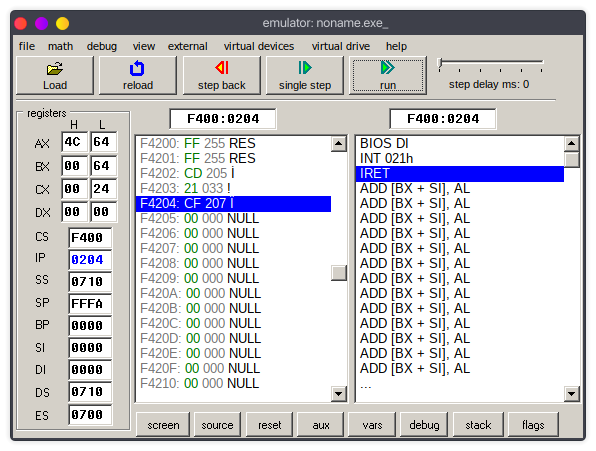
\includegraphics[width=0.90\textwidth]{img/p2/ss1.png}
	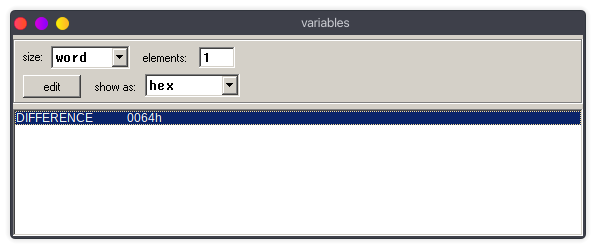
\includegraphics[width=0.90\textwidth]{img/p2/ss2.png}
\end{center}

\subsection{Result}
Two 16 bit numbers were substracted using immediate addressing mode in emu8086 and output was verified